\subsection{Cascade architecture}\label{subsec:abc-architecture}

The cascade has three tiers, as shown in Figure~\ref{fig:abc-cascade}. The first two tiers have three voters, and the final tier has a single model, which is the strongest model we have in the architecture. A voter emits, per input chunk, either no output, or one typed \texttt{AuditableSummary} object, which is a summary holding atomic findings described in Subsection~\ref{subsec:knowledge-map}, together with the metadata information needed to inspect the voter's extraction result.

\begin{figure}[htbp]
    \centering
    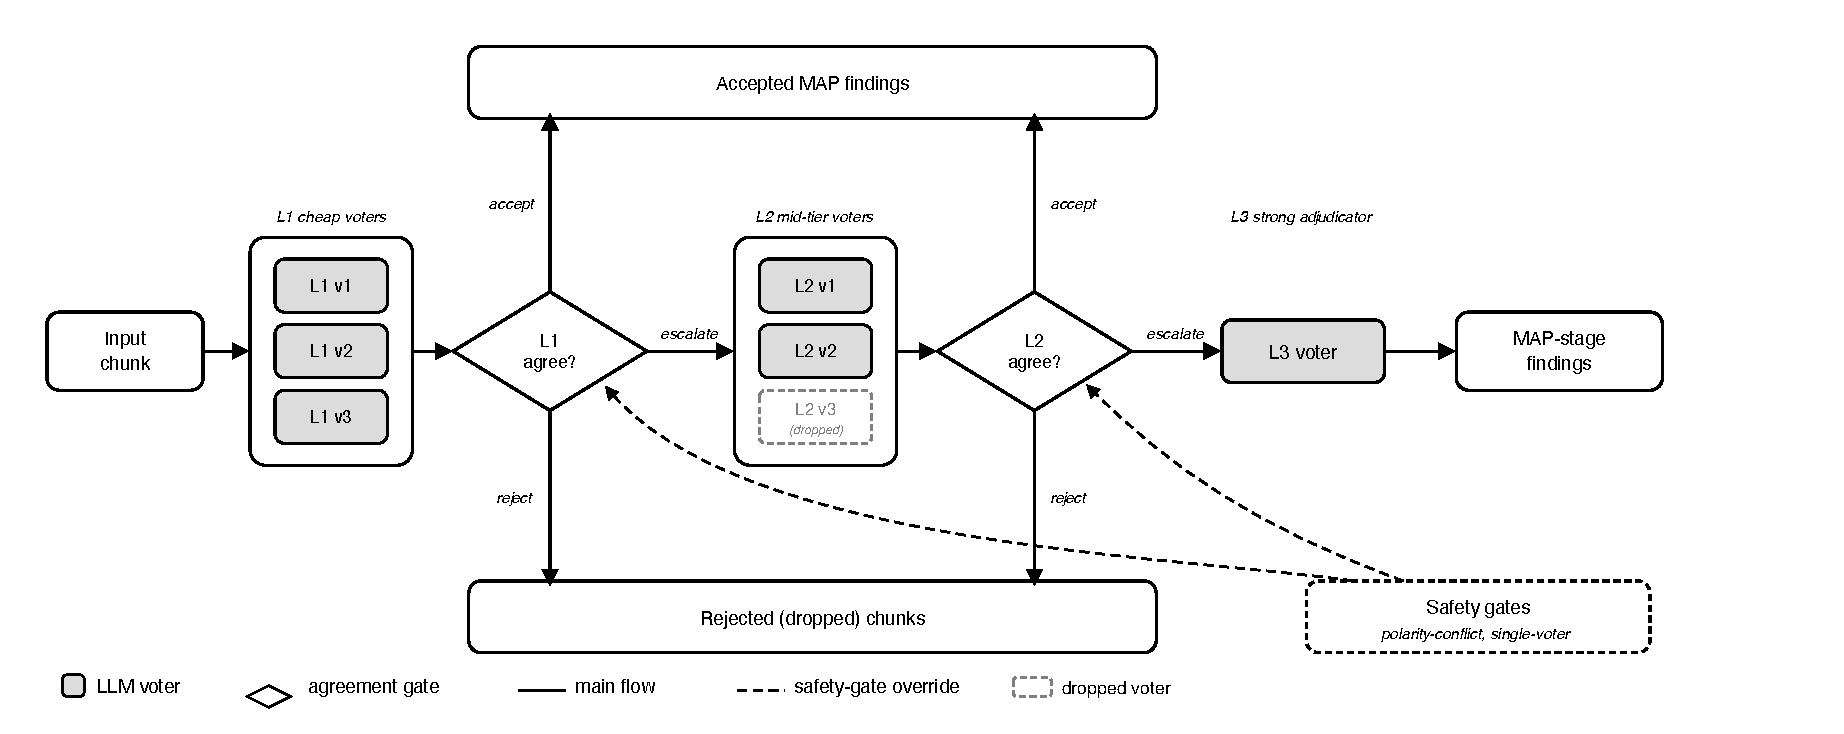
\includegraphics[width=\textwidth]{histo_thesis/figures/03_methodology/05_agreement_based_cascading/01_abc_cascade.pdf}
    \caption{Agreement-based cascading at the MAP stage.}
    \label{fig:abc-cascade}
\end{figure}

\begin{itemize}[label={}, leftmargin=1.5em, itemsep=0.4em]
    \item \textbf{Level 1 -- Cheap voters.} The first level consists of cheap models that run in parallel on every input chunk. The voter pool has models by different providers (OpenAI and Google), and different model families. When models agree at this level, this means that a genuine consensus across distinct model families was reached.
    \item \textbf{Level 2 -- Mid-tier voters.} When the L1 agreement score is not sufficient for acceptance, a second pool of moderately stronger models is invoked. At this level, a third provider, Anthropic, is added, extending the provider mix. At L2, the knowledge extraction is retried on a different and stronger set of models, instead of replaying it with the same cheap voters. 
    \item \textbf{Level 3 -- Single strong voter.} When L2 models also cannot agree on an output, the chunk escalates to the third and last level. L3 is a fallback level, which never escalates from here, and includes the strongest language model in the cascade.
\end{itemize}

The exact voter models, their configurations, and the production voter profiles are listed in the appendix configuration table. This section focuses on the architecture, rather than the concrete model names. There are two important architectural decisions made: first, voter diversity comes from using models from different providers, not from sampling variation: every production voter runs at temperature zero; second, the objects compared across voters is the typed MAP-stage output of Subsection~\ref{subsec:knowledge-map}. Agreement, therefore, is computed over structured extraction results, not raw free-text summaries.